%!TEX TS-program = xelatex
%!TEX encoding = UTF-8 Unicode

\documentclass[14pt, aspectratio=43]{beamer}
\usepackage{amsmath, fancyvrb, textcomp}
\usepackage{xcolor}
\definecolor{codecolor}{rgb}{0.0, 0.3, 0.1}
\definecolor{white}{rgb}{1,1,1}

%\usepackage{attachfile2}

% draft watermark
%\usepackage[]{draftwatermark}
%\SetWatermarkFontSize{4cm}
%\SetWatermarkColor[rgb]{1,0.8,0.8}
%\SetWatermarkAngle{30}
%\setbeamercolor{background canvas}{bg=}%transparent canvas

%% Beamer 版面配置
\mode<presentation>

%\usetheme{Pittsburgh}
%\usetheme{Singapore}
%\usecolortheme{orchid}
\usecolortheme{rose}
\useinnertheme{circles}
%\useoutertheme[subsection=false]{miniframes}


% page number shown on top-right corner
    \setbeamertemplate{headline}{%
        \vskip6pt\hspace*{\fill}\insertpagenumber\hspace*{3pt}\vspace*{-6pt}%
    }
    \setbeamercolor{headline}{fg=black!50, bg=black!50}
    \setbeamerfont{headline}{size=\footnotesize}

    \setbeamerfont{frametitle continuation}{size=\normalsize}
 

%    \setbeamercolor{postit}{bg=blue!10}
%    \setbeamertemplate{headline}
%    {%
%      \begin{beamercolorbox}[wd=1\paperwidth]{postit}
%        \vskip1pt\insertnavigation{1\paperwidth}\vskip1pt
%      \end{beamercolorbox}\vspace*{-15pt}%
%    }
%

% frametitle
    \setbeamertemplate{frametitle}{\vspace*{-0pt}\insertframetitle\hspace*{\fill}\par}
%    \setbeamercolor{frametitle}{fg=black}

\setbeamersize{text margin left=0.7cm, text margin right=0.7cm}

\let\oldfootnote\footnote
\renewcommand\footnote[1]{\hspace{-0.7em}\oldfootnote{\ignorespaces#1}\hspace{0.5em}}
\setbeamerfont{footnote mark}{size=\tiny}
\setbeamerfont{footnote}{size=\scriptsize}
\setbeamertemplate{footnote}{\textsuperscript{\insertfootnotemark}\insertfootnotetext}

\setbeamertemplate{itemize item}{\LARGE\raise-3.5pt\hbox{\textbullet}}

%\setbeamerfont{page number in head/foot}{size = \scriptsize}
%\setbeamertemplate{footline}[frame number]{}

\usefonttheme{structurebold}


\beamertemplatenavigationsymbolsempty % 去除 Beamer 導覽工具列

\DefineVerbatimEnvironment{RC}{Verbatim}{fontsize=\small, baselinestretch=0.9, samepage=true}
\DefineVerbatimEnvironment{R}{Verbatim}{fontsize=\footnotesize, frame=single, baselinestretch=0.85, samepage=true}

%% 西文字配置
\linespread{1}
\usepackage{arevmath}
\usepackage[no-math]{fontspec}

%\setmainfont[Mapping=tex-text, LetterSpace=0, BoldFont={Lato}]{Lato}
%\setsansfont[Mapping=tex-text, LetterSpace=0, BoldFont={Lato}, Scale=0.85]{Lato}
%\setmonofont[Color=codecolor, Scale=0.95, LetterSpace=-1, BoldFeatures={Color=white}, BoldFont={Consolas}]{Consolas}

\setmainfont[Mapping=tex-text, Scale=0.8, LetterSpace=-0, BoldFont={DejaVu Sans}]{DejaVu Sans}
\setsansfont[Mapping=tex-text, Scale=0.8, LetterSpace=-0, BoldFont={DejaVu Sans}]{DejaVu Sans}
\setmonofont[Color=codecolor, Scale=0.8, LetterSpace=-2, BoldFeatures={Color=white}, BoldFont={DejaVu Sans Mono}]{DejaVu Sans Mono}

\usefonttheme{professionalfonts}


%% 中文字配置
\newcommand{\nbs}{\hskip3pt plus 1pt minus 1pt}
\usepackage[
  CJKmath=true, indentfirst=false, PunctStyle={quanjiao},
  CheckSingle=false, Verb=true, AutoFallBack=true, AutoFakeBold=false, AutoFakeSlant=false, 
  CJKglue = {\hskip-0.4pt plus 2pt}, CJKecglue = {\nbs}
]{xeCJK}
\setCJKmainfont[Scale=0.95, BoldFont={cwTeX Q Hei Bold}, LetterSpace=0]{cwTeX Q Hei}
\setCJKmonofont[Scale=0.95, BoldFont={cwTeX Q Hei Bold}, LetterSpace=-0, Color=codecolor]{cwTeX Q Yuan}


\title{初學R語言的60分鐘}
\author{廖鎮磐 \texttt{<andrew.43@gmail.com>}}
\institute{東海大學生命科學系}
\date{2015年台灣生態研究網年會 -- 2015年3月14日於蓮華池研究中心}
\hypersetup{
    bookmarks=true,         % show bookmarks bar?
    unicode=true,           % non-Latin characters in Acrobat’s bookmarks
    pdftoolbar=true,        % show Acrobat’s toolbar?
    pdfmenubar=true,        % show Acrobat’s menu?
    pdffitwindow=false,     % window fit to page when opened
    pdfstartview={FitH},
    pdfpagelayout={OneColumn},
%    pdfpagemode={FullScreen},
    pdfpagemode={UseOutlines},
    pdfdisplaydoctitle=true,
    pdfinfo={License={Attribution-ShareAlike 4.0 International}},
    pdftitle={初學R語言的60分鐘},
    pdfauthor={廖鎮磐 (Chen-Pan Liao) <andrew.43@gmail.com>},
    pdfsubject={針對R語言的初學者所設計的教學投影片。主題包括建立R操作環境、了解R的函數使用方法、資料讀取、常見的統計分析與繪圖。},
    pdfkeywords={R語言, 投影片, 初學},
    pdflang={zh-TW},
    xetex
}

\setbeamertemplate{title page}{
  \vskip0pt plus 1filll
    \LARGE{\bfseries\usebeamercolor[fg]{title}初學\hspace{0.2em}
\includegraphics[width=3cm]{Rlogo-novo.png}\hspace{0.2em}語言的60分鐘}\\[8pt]
    \normalsize{廖鎮磐 \texttt{<andrew.43@gmail.com>}\\東海大學生命科學系}\\[10pt]
    \normalsize{2015年台灣生態研究網年會\\ 2015年3月14日於蓮華池研究中心}
    \vskip0pt plus 0.5filll
    {\scriptsize
        \parbox[c]{2.7cm}{% 
          
\includegraphics[width=2.7cm]{cc.pdf}%
        }\hspace{6pt}%
        \parbox[c]{8.2cm}{% 
           © 2015 廖鎮磐(Chen-Pan Liao)\\[-1pt]
	   本文件採用姓名標示-相同方式分享 4.0 國際授權(CC BY-SA 4.0)。\footnote{詳情請見 \url{http://creativecommons.org/licenses/by-sa/4.0/deed.zh_TW}。}\\[-1pt]
	   歡迎下載本投影片及資料檔案。\footnote{\url{https://www.dropbox.com/sh/7p9cluglptyk25a/AAAmPWrSMVf_tC9-cL4JSscCa?dl=0}}
	 }% 
	 \vspace{10pt}
    }
}






\AtBeginSection[] {
  \begin{frame}
    \frametitle{大綱}
    \tableofcontents[currentsection]
  \end{frame}
  \addtocounter{framenumber}{-1}
} 

\begin{document}
\xeCJKOffVerbAddon


\begin{frame}
\titlepage
\end{frame}

\begin{frame}
\frametitle{大綱}
\tableofcontents
\end{frame}

\section{R簡介與操作環境}\subsection{}

\begin{frame}{今天主題$\cdots\cdots$}

\begin{block}{目標}
\begin{itemize}
\item 不怕害使用R這類以文字指令進行的工作方式。
\item 如何自己救自己。
\item 如何請別人救自己。
\item 實作一些常見的統計分析與繪圖。
\end{itemize}
\end{block}

\begin{block}{預設聽眾}
\begin{itemize}
\item 修過至少3學分的統計學。
\item 從沒使用過R或其它統計軟體。
\item 從沒學過任何程式語言。
\end{itemize}
\end{block}

\end{frame}




\begin{frame}{R的特色}
\framesubtitle{為什麼我選擇R?}
\begin{itemize}
\item 自由、免費、跨平台。
\item 是一種「程式語言」,像Python、Perl、JAVA等。
\item 是一種「統計工具」,像SAS、SPSS等。
\item 強大的視覺化工具,畫專業的圖,但需要經驗。
\item 套件豐富,不同自己重新寫程式。
\end{itemize}
\end{frame}

\begin{frame}[fragile]{安裝R語言}
\begin{enumerate}
\item 到達 \url{http://www.r-project.org/}
\item 點選Download, Packages (CRAN) \\
\item 選擇作業平台
\end{enumerate}
	\begin{center}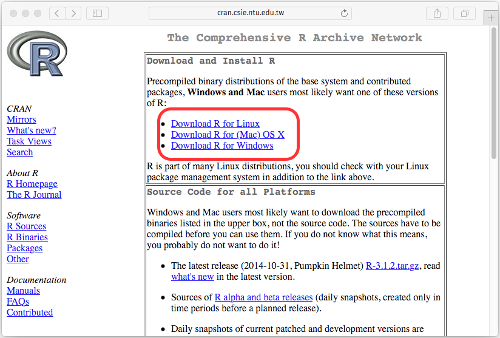
\includegraphics[width=0.6\textwidth]{downloadR.png}\end{center}
\end{frame}

\begin{frame}[fragile]{選用適當的R程式編輯器}
\begin{itemize}
\item 建議以純文字編輯器撰寫R程式碼,並儲存成「\verb+.R+」檔。
\item 「語法多色支援」、「語法提示」、「即時執行」等功能,增加撰寫效率。
\item 支援R語言的編輯器很多,有興趣請自行試用。
\begin{description}[longest item]
	\item [RStudio] 強大、整合性高、專為R程式員設計。\footnote{\url{http://www.rstudio.com/}}
	\item [Notepad++] 老字號的純文字編輯器,有和R相配合的外掛。\footnote{\url{http://notepad-plus-plus.org/}}
	\item [Atom] 與GitHub配合度高。\footnote{\url{https://atom.io/}}
\end{description}
\end{itemize}
\end{frame}


\begin{frame}[fragile]{初次見面:R是計算機}
\begin{columns}
\column{0.22\textwidth}
\begin{verbatim}
> 2.4 + 42
[1] 44.4
> 4 ^ 2
[1] 16
> sqrt(100)
[1] 10
> 100 ^ 0.5
[1] 10
\end{verbatim}

\column{0.22\textwidth}
\begin{verbatim}
> a <- 1
> a
[1] 1
> 1 -> b
> b
[1] 1
> a + b
[1] 2
\end{verbatim}

\column{0.45\textwidth}
\begin{verbatim}
> m <- c(3, 6, 4)
> n <- c(1, 2, 3)
> m + n
[1] 4 8 7
> m - n
[1] 2 4 1
> m * n
[1]  3 12 12
> m / n
[1] 3.000 3.000 1.333
\end{verbatim}


\end{columns}
\end{frame}


%\begin{frame}[fragile]{Q\&A的時間到囉}
%\begin{itemize}
%\item[Q] 如何找能做某件事的套件?
%\item[A] 請Google大神幫你找最快。真的。
%\end{itemize}
%\end{frame}

\section{R的函數}\subsection{}

\begin{frame}[fragile]{什麼是程式語言的函數(function)}


\begin{itemize}
\item 程式語言的函數提供一個特定的功能,可以輸入引數(輸入值)並取得回傳值(輸出值)。
\item 操作R的過程,幾乎就是使用各種function的過程。
%\item 若需要進行某一套程式多次,可以將之改寫成函數以利重覆使用。
\end{itemize}

\begin{block}{使用某函數的語法通則}
\verb+函數名(第一引數名 = 某值, 第二引數名 = 某值, ...)+ 
\end{block}

\begin{itemize}
\item 試試看\nbs\verb+seq(from = 0, to = 9)+\nbs{}的回傳值是什麼?
\item 用中文說明上面的程式:「在\nbs\verb+seq()+\nbs{}這個function中,第一個引數名為\nbs\verb+from+,表示起始值,其值為0;第二個引數名為\nbs\verb+to+,表示終點值,其值是9。」
\end{itemize}
\end{frame}



\begin{frame}[fragile]{函數的使用手冊}
\begin{itemize}
\item 觀看某個函數的使用手冊:\verb+?函數名+\nbs{}或\nbs\verb+help(函數名)+。
\item 請看看\nbs\verb+?seq+。
\item 使用手冊中都有以下資訊:
\begin{description}[longest item]
	\item [Description] 函數的功能。
	\item [Usage] 基本語法,包括了引數的順序和預設值。
	\item [Arguments] 引數的細節。
	\item [Details] 函數的詳細內容。
	\item [Value] 回傳值的內容。
	\item [See Also] 其它相關的函數。
	\item [Examples] 使用範例。
\end{description}
\end{itemize}
\end{frame}



\begin{frame}[fragile]{引數的預設值}

\begin{block}{\texttt{seq()} 的基本語法}
\verb+seq(from = 1, to = 1, ...)+ \\
\end{block}
\begin{itemize}
\item 在使用手冊中可以看出:
  \\ 第一個引數\nbs\verb+from+\nbs{}的預設值是 1。
  \\ 第一個引數\nbs\verb+to+\nbs{}的預設值是 1。
\item 使用者未定義時採用的值,就是預設值。
\item 方便快速使用。
\item 例如:\\
  \verb+seq(from = 10)+\nbs{}和 \\
  \verb+seq(from = 10, to = 1)+\nbs{}是相等的。
\end{itemize}
\end{frame}


\begin{frame}[fragile]{引數的順序}

\begin{block}{\texttt{seq()}的基本語法}
\verb+seq(from = 1, to = 1, ...)+ \\
\end{block}

\begin{itemize}
\item 當明確指定引數名時,引數的順序無所謂。例如:\\ \verb+seq(from = 0, to = 9)+\nbs{}和 \\ \verb+seq(to = 9, from = 0)+\nbs{}同義。
\item 當引數的順序與該函數要求的順序相同時,可以省略引數名。例如:\\ \verb+seq(from = 0, to = 9)+\nbs{}可以省略為 \\ \verb+seq(0, 9)+\nbs{}的形式。
\end{itemize}
\end{frame}


\begin{frame}[fragile]{引數的綜合練習}

\begin{block}{\texttt{seq()}的基本語法}
\verb+seq(from = 1, to = 1, ...)+ \\
\end{block}

試回答下列程式的回傳值為何?
\begin{itemize}
\item \verb+seq(from = 3, to = 1)+
\item \verb+seq(3, to = 1)+
\item \verb+seq(from = 3, 1)+
\item \verb+seq(3, 1)+
\item \verb+seq(to = 1, from = 3)+
\end{itemize}
\end{frame}



\begin{frame}[fragile]{Q\&A的時間又到囉}
\begin{itemize}
\item[Q] 成千上萬的函數哪學得完?
\item[A] 不用學完!沒人學得完!學常用的就好。
\end{itemize}
\begin{itemize}
\item[Q] 函數的使用手冊看不懂耶。
\item[A] 我也常看不懂。儘量看,多嘗試,特別是Example部份。
\end{itemize}
\begin{itemize}
\item[Q] 如何找能做某件事的函數?
\item[A] 請Google大神幫你找最快。真的。
\end{itemize}
\end{frame}


\section{資料的讀取與整理}\subsection{}


\begin{frame}[fragile]{檔案下載}
\begin{enumerate}
\item 至 \url{http://goo.gl/foAeaq} 以下載檔案:
\begin{description}[longest item]
%\item [\texttt{2015RforBeginnerSlide.pdf}]本投影片
\item [\texttt{exam.xlsx}]例範資料
\item [\texttt{text.xlsx}]練習資料
\end{description}

\item 在C disk 下創建一個\nbs\verb+LearnR2015+\nbs{}資料夾,並將檔案置入該資料夾中。
\end{enumerate}
%\begin{center}
%\Huge\url{http://goo.gl/YRCOaN}\\
%
\includegraphics[width=2.5in]{url-dropbox.pdf}
%\end{center}
\end{frame}


\begin{frame}[fragile]{讀取CSV資料檔案}
\begin{enumerate}
\item 開啟\nbs\verb+exam.xlsx+,注意第一列必需有一列「變數名」。
\item 另存新檔 $\rightarrow$ 檔名為「exam」,類型為「CSV」,儲存在相同資料夾中。
\item \verb+getwd()+\nbs{}顯示目前R所在的路徑。
\item \verb+setwd("C:/LearnR2015")+\nbs{}到達該資料夾。
\item \verb+dt <- read.csv("exam.csv")+\nbs{}或是 \\
      \verb+dt <- read.csv("C:/LearnR2015/exam.csv")+\nbs{}以讀取該檔成為一個資料框(data frame),並取名為 \verb+dt+。\\
\end{enumerate}
\end{frame}


\begin{frame}[fragile]{提取特定變數(欄)}
\verb+dt+\nbs{}的結果是什麼?
\begin{R}
> dt
  ID Gender Group Literature Science
1 23      m     A         36      63
...
\end{R}

如何取得Science變數?直接輸入\nbs\verb+Science+\nbs{}是不行的,因為它是在\nbs\verb+dt+\nbs{}裡的變數。
\begin{itemize}
\item \verb+dt$Science+\nbs{}意思是「dt裡的Science變數」
\item \verb+dt[ , 5]+\nbs{}意思是「dt裡的第5欄變數」
\item \verb+attach(dt)+\nbs{}可使dt的所有變數傳至表層。
\end{itemize}
\end{frame}


\begin{frame}[fragile]{提取特定重覆數(列)}
\begin{itemize}
\item \verb+dt[3 , ]+ \\ 取得dt裡的第3列資料
\item \verb+dt[c(3, 6) , ]+ \\ 取得dt裡的第3及第6列資料
\item \verb+subset(dt, Gender == "m")+ \\ 取得Gender是m的資料。
\item \verb+subset(dt, Science >= 60)+ \\ 取得Science大於等於60的資料。
%\item \verb+subset(dt, Gender == "m" | Science >= 60)+ \\ 取得Gender是m \alert{或} Science大於等於60的資料。
%\item \verb+subset(dt, Gender == "m" & Science >= 60)+ \\ 取得Gender是m \alert{且} Science大於等於60的資料。
\end{itemize}
\end{frame}

\begin{frame}[fragile]{Q\&A的時間又到囉}
\begin{itemize}
\item[Q] 可否直接讀取xlsx檔?\\
\item[A] 可以!請日後自行研究\nbs\verb+xlsx+\nbs{}這個套件。
\end{itemize}
\begin{itemize}
\item[Q] 中文資料怎麼辦?\\
\item[A] 資料中有中文可能是件麻煩事,都可以解決,但初學者還是避免比較方便。
\end{itemize}
\begin{itemize}
\item[Q] 可不可以資料排序?\\
\item[A] 可以!請日後自行研究\nbs\verb+order()+\nbs{}和\nbs\verb+sort()+。
\end{itemize}
\end{frame}


\section{統計分析與繪圖}\subsection{}

\begin{frame}[fragile]{描述性統計}
\begin{block}{常見的描述性統計函數}
\verb+length(dt$Science)   #個數+ \\
\verb+mean(dt$Science)     #平均數+ \\
\verb+sd(dt$Science)       #標準偏差+ \\
\verb+quantile(dt$Science) #百分位數+ \\
\end{block}

如果要求各組的描述性統計呢?使用\nbs\verb+tapply()+。
\begin{block}{\texttt{tapply()}的基本語法}
\verb+tapply(變數, 分組因子, 運算函數, ...)+
\end{block}
例如,要計算Science在不同Gender內的平均數:\\
\verb+tapply(dt$Science, dt$Gender, mean)+\\
%或是用\verb+subset()+切出子集,例如\\
%\verb+mean( subset(dt, Gender == "m")$Science )+ \\
\end{frame}

\begin{frame}[fragile, allowframebreaks]{單樣本\emph{T}檢驗}

目標:檢驗Science的平均是否為60。
\begin{block}{\texttt{t.test()}的基本語法}
\verb+t.test(資料, alternative = "t" 或 "l" 或 "g",+
\verb+       mu = 假說平均數, ...)+
\end{block}
\begin{RC}
> # 雙尾:
> t.test(dt$Science, alternative = "t", mu = 60) 
> # 右單尾:
> t.test(dt$Science, alternative = "g", mu = 60) 
> # 左單尾:
> t.test(dt$Science, alternative = "l", mu = 60) 
\end{RC}

\framebreak

\begin{RC}
> t.test(dt$Science, mu = 60)
\end{RC}
\begin{R}
	One Sample t-test

data:  dt$Science
t = 1.5393, df = 8, p-value = 0.1623
alternative hypothesis: true mean is not equal to 60
95 percent confidence interval:
 54.63219 86.92336
sample estimates:
mean of x 
 70.77778 
\end{R}
\end{frame}

\begin{frame}[fragile, allowframebreaks]{成對樣本\emph{T}檢驗}
目標:檢驗Literature和Science差之平均是否為0。
\begin{block}{\texttt{t.test()}的基本語法}
\verb+t.test(資料1, 資料2,+
\verb+       alternative = "t" 或 "l" 或 "g",+
\verb+       mu = 假說中配對差的平均數, pair = T, ...)+
\end{block}
\begin{RC}
> # 預設雙尾;預設平均差為零
> t.test(dt$Literature, dt$Science, pair = T)
\end{RC}

\framebreak

\begin{RC}
> t.test(dt$Literature, dt$Science, pair = T)
\end{RC}
\begin{R}
	Paired t-test

data:  dt$Literature and dt$Science
t = -4.2126, df = 8, p-value = 0.002945
alternative hypothesis: true difference in means is not equal to 0
95 percent confidence interval:
 -17.193365  -5.028857
sample estimates:
mean of the differences 
              -11.11111 
\end{R}
\end{frame}


\begin{frame}[fragile, allowframebreaks]{獨立雙樣本\emph{T}檢驗}
目標:檢驗二種Gender的Literature之平均是否相等。
%\verb+tapply(dt$Literature, dt$Gender, mean) #分組平均+
%\verb+tapply(dt$Literature, dt$Gender, sd)   #分組標準差+
\begin{block}{\texttt{t.test()}的基本語法}
\verb+t.test(資料一, 資料二, mu = 假說中平均數的差,+\\
\verb+       alternative = "t" 或 "l" 或 "g",+\\
\verb+       var.equal = T 或 F, ...)+
\verb+t.test(應變數 ~ 二類類別因子,+\\
\verb+       data = 資料框, ...)+
\end{block}
\begin{RC}
> t.test(subset(dt, Gender == "m")$Literature,
+        subset(dt, Gender == "f")$Literature,
+        var.equal = T)
> t.test(Literature ~ Gender, data = dt, var.equal = T)
\end{RC}

\framebreak

\begin{RC}
> t.test(Literature ~ Gender, data = dt, var.equal = T)
\end{RC}
\begin{R}
	Two Sample t-test

data:  Literature by Gender
t = -0.8823, df = 7, p-value = 0.4069
alternative hypothesis: true difference in means is not equal to 0
95 percent confidence interval:
 -43.60845  19.90845
sample estimates:
mean in group f mean in group m 
          54.40           66.25 
\end{R}
\end{frame}

\begin{frame}[fragile]{盒形圖}

\begin{block}{\texttt{boxplot()}的基本語法}
\verb+boxplot(應變數 ~ 類別因子, data = 資料框, ...)+
\end{block}

\begin{RC}
> boxplot(Literature ~ Gender, data = dt, 
+         ylab = "Literature score", xlab = "Gender")
\end{RC}

\begin{center}
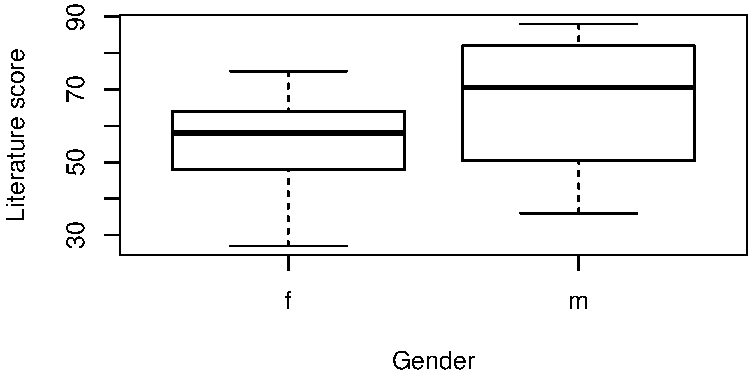
\includegraphics[width=0.75\textwidth]{Rplot-two-group.pdf}
\end{center}
\end{frame}

%pdf("Rplot-two-group.pdf", width=5, height=2.5)
%par(mar=c(4,4,0.5,0.1))
%boxplot(Literature ~ Gender, data = dt, 
%  ylab = "Literature score", xlab = "Gender")
%dev.off()

\begin{frame}[fragile, allowframebreaks]{單因子變異數分析}
目標:檢驗三種Group的Literature之平均是否相等,並進行Tukey事後檢驗。

\begin{block}{\texttt{aov()}和\texttt{TukeyHSD()}的基本語法}
\verb+aov(應變數 ~ 三組以上類別自變數, +\\
\verb+    data = 資料框, ...)+\\
\verb+TukeyHSD(aov物件, "分組因子", ...)+
\end{block}
\begin{RC}
> fit.1 <- aov(Literature ~ Group, data = dt)
> summary(fit.1) # Type I sum of square
> TukeyHSD(fit.1, "Group")
\end{RC}


\framebreak

\begin{RC}
> fit.1 <- aov(Literature ~ Group, data = dt)
> summary(fit.1)
\end{RC}
\begin{R}
            Df Sum Sq Mean Sq F value Pr(>F)
Group        2    2.7     1.3   0.003  0.997
Residuals    6 3115.3   519.2               
\end{R}
\begin{RC}
> TukeyHSD(fit.1, "Group")
\end{RC}
\begin{R}
  Tukey multiple comparisons of means
    95% family-wise confidence level

Fit: aov(formula = Literature ~ Group, data = dt)

$Group
         diff       lwr      upr     p adj
B-A 0.6666667 -56.41875 57.75209 0.9992924
C-A 1.3333333 -55.75209 58.41875 0.9971738
C-B 0.6666667 -56.41875 57.75209 0.9992924
\end{R}
\end{frame}

\begin{frame}[fragile]{盒形圖}

\begin{block}{\texttt{boxplot()}的基本語法}
\verb+boxplot(應變數 ~ 類別因子, data = 資料框, ...)+
\end{block}

\begin{RC}
> boxplot(Literature ~ Group, data = dt, 
+         ylab = "Literature score", xlab = "Group")
\end{RC}

\begin{center}
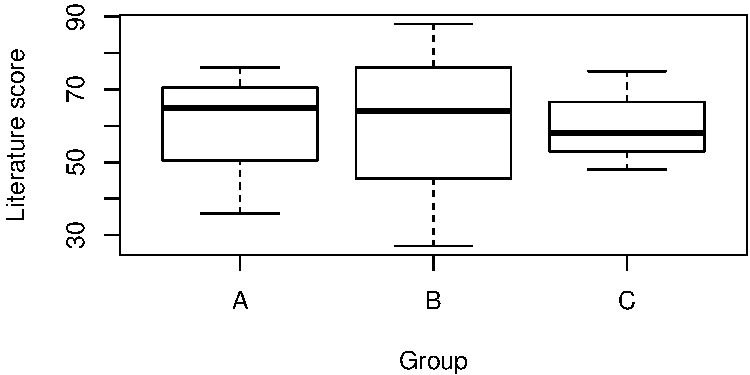
\includegraphics[width=0.75\textwidth]{Rplot-three-group.pdf}
\end{center}
\end{frame}

%
%pdf("Rplot-three-group.pdf", width=5, height=2.5)
%par(mar=c(4,4,0.5,0.1))
%boxplot(Literature ~ Group, data = dt, 
%  ylab = "Literature score", xlab = "Group")
%dev.off()


\begin{frame}[fragile, allowframebreaks]{簡單線性迴歸}
目標:建立Science對應Literature的簡單線性迴歸模型,並檢驗斜率是否為零。
\begin{block}{\texttt{lm()}的基本語法}
\verb+lm(應變數 ~ 連續自變數, data = 資料框, ...)+
\end{block}
\begin{RC}
> fit.2 <- lm(Literature ~ Science, data = dt)
> summary(fit.2)
> anova(fit.2) # Type I sum of square
\end{RC}

\framebreak

\begin{RC}
> fit.2 <- lm(Literature ~ Science, data = dt); 
> summary(fit.2)
\end{RC}
\begin{R}
Call:
lm(formula = Literature ~ Science, data = dt)

Residuals:
    Min      1Q  Median      3Q     Max 
-16.894  -1.085   2.494   4.269   8.113 

Coefficients:
            Estimate Std. Error t value Pr(>|t|)    
(Intercept)  -1.9625     9.8294  -0.200 0.847422    
Science       0.8707     0.1337   6.511 0.000331 ***
---

Residual standard error: 7.946 on 7 degrees of freedom
Multiple R-squared:  0.8583,	Adjusted R-squared:  0.838 
F-statistic: 42.39 on 1 and 7 DF,  p-value: 0.0003308
\end{R}

\framebreak

\begin{RC}
> anova(fit.2)
\end{RC}
\begin{R}
Analysis of Variance Table

Response: Literature
          Df  Sum Sq Mean Sq F value    Pr(>F)    
Science    1 2676.08 2676.08  42.389 0.0003308 ***
Residuals  7  441.92   63.13                      
\end{R}
\end{frame}

\begin{frame}[fragile, allowframebreaks]{簡單線性相關}
目標:計算Science與Literature的簡單線性相關係數是否為零。
\begin{block}{\texttt{cor.test()}的基本語法}
\verb+cor.test(資料一, 資料二,+
\verb+         alternative = "t" 或 "l" 或 "g", ...)+
\verb#cor.test( ~ 資料一 + 資料二, data = 資料框, ...)#
\end{block}
\begin{RC}
> cor.test(dt$Literature, dt$Science)
> cor.test(~ Literature + Science, data = dt)
> cor.test(~ Science + Literature, data = dt)
\end{RC}

\framebreak

\begin{RC}
> cor.test(dt$Literature, dt$Science)
\end{RC}
\begin{R}
	Pearson's product-moment correlation

data:  dt$Literature and dt$Science
t = 6.5107, df = 7, p-value = 0.0003308
alternative hypothesis: true correlation is not equal to 0
95 percent confidence interval:
 0.6817766 0.9847014
sample estimates:
      cor 
0.9264278
\end{R}
\end{frame}

\begin{frame}[fragile, allowframebreaks]{散佈圖}

\begin{block}{\texttt{coef()}的基本語法}
\verb+coef(lm物件, ...)+  \# 取出各迴歸係數
\end{block}

\begin{block}{\texttt{plot.formula()}和\texttt{abline()}的基本語法}
\verb+plot(縱軸資料 ~ 橫軸資料, data = 資料框, ...)+\oldfootnote{\texttt{plot.formula()}可簡寫成\texttt{plot()}。}\\
\verb+abline(a = coef(迴歸物件)[1],+\\
\verb+       b = coef(迴歸物件)[2],+\\
\verb+       lty, col, ...) # 畫上迴歸線 +
\end{block}

\begin{RC}
> plot(Literature ~ Science, data = dt)
> abline(a = coef(fit.2)[1], b = coef(fit.2)[2], lty = 3)
\end{RC}

\framebreak

\begin{RC}
> plot(Literature ~ Science, data = dt)
> abline(a = coef(fit.2)[1], b = coef(fit.2)[2], lty = 3)
\end{RC}

\begin{center}
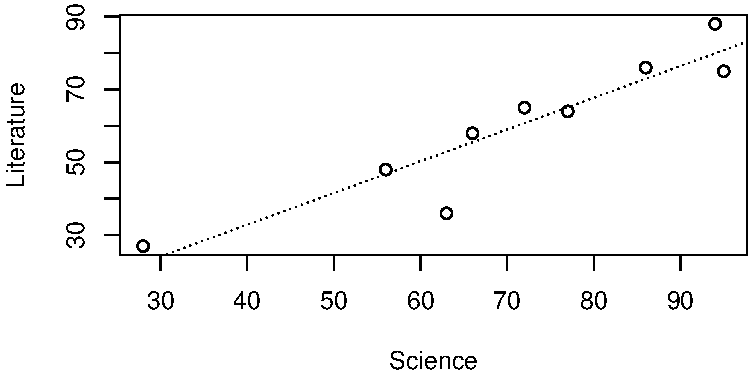
\includegraphics[width=0.75\textwidth]{Rplot-sct.pdf}
\end{center}
\end{frame}

%
%pdf("Rplot-sct.pdf", width=5, height=2.5)
%par(mar=c(4,4,0.5,0.1))
%fit <- lm(Literature ~ Science, data = dt)
%plot(Literature ~ Science, data = dt)
%abline(a = coef(fit)[1], b = coef(fit)[2], lty = 3)
%dev.off()




%\begin{frame}[fragile]{卡方適合度檢驗}
%\end{frame}

%\begin{frame}[fragile]{卡方獨立性檢驗}
%\end{frame}


\begin{frame}[fragile]{Q\&A的時間又到囉}
\begin{itemize}
\item[Q] 我怎麼知道我做對了?
\item[A] 拿出你的統計學課本的例題,用R做做看。
\end{itemize}
\begin{itemize}\item[Q] R畫的圖想做更多調整$\ldots\ldots$
\item[A1] 這件工作不是非常容易,需要經驗。有空看看\nbs\verb+par()+\nbs{}和\nbs\verb+plot()+\nbs{}的使用手冊。
\item[A2] 初學者可以先用 R 畫個大概的樣子,再以其它圖片編輯軟體後製。參考\nbs\verb+png()+、\verb+pdf()+、\verb+svg()+\nbs{}等方法來輸出圖檔。
\end{itemize}
\end{frame}



\section{學習心得與討論資源}\subsection{}

\begin{frame}{阿盤的個人學習心得}
\begin{itemize}
\item 修習使用R的課。
\item 多「玩」。把函數裡的 Example 玩一玩、改一改。
\item 肯問人。逛逛網路教學和論壇。
\item 買(可能不只一本)書。
\item 拿出統計學課本的例題,用R做做看。
\item 做過的程式碼要建檔,方便日後使用。
\item 卡關時,先用英文問Google大神。
\item 做出答案時,不要直接相信這是正解,應該以專業人士、書籍、網頁資料驗證。
\end{itemize}
\end{frame}


\begin{frame}{中文書籍推薦}
繁體中文書非常少,但簡體中文書不少。去圖書館或書局翻翻。能看懂有收穫就有參考價值。初學程式語言者應該都需要一本。
\begin{itemize}
\item 《R軟體:應用統計方法》陳景祥著,東華出版社。\\ 對初學者很有幫助的一本。R語言和統計學併重。
\item 《R 錦囊妙計》 Paul Teetor著,張夏菁譯,歐萊禮出版社。\\ 前半本內容是R語言,後半本是以R進行統計工作。
\item {\CJKfontspec[Scale=0.88]{WenQuanYi Micro Hei}《R语言实用教程》薛毅、陈立萍著,清华大学出版社。}
\item {\CJKfontspec[Scale=0.88]{WenQuanYi Micro Hei}《统计建模与R软件》薛毅、陈立萍著,清华大学出版社。} \\ 以數理統計為主,R語言實作為輔。
\end{itemize}
\end{frame}

\begin{frame}{英文書籍推薦}
英文書選擇極多。我推薦以下幾本我喜歡或值得閱讀的。
\begin{itemize}
\item ``Biostatistical Design and Analysis Using R: A Practical Guide'' by Murray Logan. Wiley-Blackwell Press.\\ 實驗設計和R並重,非常推薦。
\item ``The R Book, 2\textsuperscript{nd} Edition'' by Michael J.~Crawley. Wiley Press. \\ 較不易閱讀,但仍值得細讀。R語言和統計併重。
\item ``A First Course in Statistical Programming with R'' by W.~John Braun \& Duncan J.~Murdoch. Cambridge University Press. \\ 易讀。統計學基礎內容為主,但實驗設計部份少。
\end{itemize}
\end{frame}


\begin{frame}{網路教學}
\begin{itemize}
\item 《R 演習室》\makeatletter @ \makeatother youtube.com\oldfootnote{\url{https://www.youtube.com/playlist?list=PL5AC0ADBF65924EAD}} \\ 針對初學者的 R 視訊教學系列。有廣告(歡迎多看幾秒),但有提供影片載點。
\item \url{http://www.r-software.org/home} \\ 中華R軟體學會。收錄許多中文影片與中文教學,內容豐富,亦適合初學者。
\item ``Quick-R''by Robert I.~Kabacoff\oldfootnote{\url{http://www.statmethods.net/}}\\ 我常用的速查網站。
\item 英文的的網路教學非常多,請自行搜尋「R turorial」。
\end{itemize}
\end{frame}


\begin{frame}{網路討論區}
\begin{itemize}
\item PTT的R\_Language板 \\ 路徑:戰略高手 $\rightarrow$ CompScience $\rightarrow$ R\_Language\\ 對初學者友善。
\item (中文的)R軟體使用者論壇\oldfootnote{\url{https://groups.google.com/forum/?hl=zh-TW\#!forum/taiwanruser}}
\item Tag ``R''  \makeatletter @ \makeatother stackoverflow.com\oldfootnote{\url{http://stackoverflow.com/questions/tagged/r}}
\end{itemize}
\end{frame}



\begin{frame}[fragile]{R的套件}
\begin{block}{什麼是套件(package)?}
安裝在R系統裡的外掛,讓你「不用重新造輪子」。
\end{block}

\begin{block}{如何安裝、更新及引入套件?}
\begin{itemize}
\item 連上網路之後,輸入\nbs\verb+install.packages("套件名稱")+\nbs{}可以安裝某套件
\item 在已安裝某套件之後,輸入\nbs\verb+library(套件名稱)+\nbs{}可引入該套件,之後才可以使用它的功能。
\item 連上網路之後,輸入\nbs\verb+update.packages()+\nbs{}可以更新所有已安裝套件。
\end{itemize}
\end{block}

%\begin{block}{練習}
%安裝一個名叫「\verb+vegan+」的套件,並將之引入R中。
%\end{block}
\end{frame}

\begin{frame}[fragile]{R的官方套件庫}
R官方收錄有六千多個的套件,\footnote{\url{http://cran.r-project.org/web/packages/available_packages_by_name.html}}可直接以\nbs\verb+install.packages()+\nbs{}安裝。
\begin{block}{我常用的套件}
\begin{itemize}
\item (一般/廣義)線性模型:gmodels、lmtest、aod
\item 混合模型:lme4、nlme、MCMCglmm
\item 蒙地卡羅、隨機化:permute、boot
\item 多變量、群落生態、生物多樣性:vegan
\end{itemize}
\end{block}
\end{frame}


\begin{frame}[fragile]{Q\&A的時間又到囉}
\begin{itemize}
\item[Q] 如何找能做某件事的套件?
\item[A] 請Google大神幫你找最快。真的。
\end{itemize}
\begin{itemize}
\item[Q] 阿盤學多久才叫「上手」、「有生產力」?
\item[A] 自學半年以上,但我今天就要把八成功力都傳給你了!
\end{itemize}
\begin{itemize}\item[Q] 聽到這裡,我想認輸了$\ldots\ldots$我想重回用滑鼠搞定的世界。
\item[A] 只要是適合自己的工具,就是好工具。
\end{itemize}
\end{frame}

\begin{frame}[fragile]{今日的總複習}
\begin{itemize}
\item 建立一個(適合自己的)R工作環境
\item 了解R的函數與如何閱讀其使用手冊
\item R如何讀取並整理資料
\item 練習常見的統計方法
\item 讓自己更厲害的資源
\end{itemize}

\large
\begin{verbatim}
> cat("Have wonderful R experiences!\n")
> q()
\end{verbatim}

%\textattachfile[appearance=false, mimetype="application/vnd.openxmlformats-officedocument.spreadsheetml.sheet"]{exam.xlsx}{}
%\textattachfile[appearance=false, mimetype="application/vnd.openxmlformats-officedocument.spreadsheetml.sheet"]{nation-data.xlsx}{}
\end{frame}



\section{試練窟}\subsection{}

\begin{frame}[shrink=8, fragile]{按今日課程試著完成以下練習}
\begin{enumerate}
\item 想辦法以R讀取\nbs\verb+nation-data.xlsx+\nbs{}的內容並命名為\nbs\verb+mydt0+\nbs{}資料框。以檔案中所有國家為樣本完成以下分析。
\item 利用配對樣本\emph{T}檢驗,考驗\nbs\verb+Mortality.rate.child+\nbs{}之平均是否顯著高於\nbs\verb+Mortality.rate.newborn+\nbs{}之平均。提示:不是雙尾檢驗。
\item 以\nbs\verb+GDP.10000+\nbs{}為組別,計算\nbs\verb+HIV.rate+\nbs{}在各組的平均值和標準偏差,並利用獨立雙樣本\emph{T}檢驗比較組間的平均是否顯著不等,以及繪製對應的盒形圖。
\item 以\nbs\verb+Continent+\nbs{}為組別,計算\nbs\verb+Age.ave+\nbs{}在各組的平均值和標準偏差,並利用單因子變異數分析比較組間的平均差異是否顯著不等,以及繪製對應的盒形圖。
\item 以\nbs\verb+HIV.rate+\nbs{}為反應變數(應變數),\verb+Age.ave+\nbs{}為解釋變數(自變數),建立簡單線性迴歸模型,並檢驗斜率及相關係數是否顯著不為零,以及繪製對應之散佈圖。
\end{enumerate}
\end{frame}

\begin{frame}{ }
\begin{center}
{\Huge 以下是參考解答\\ \normalsize 防雷一下}
\end{center}
\end{frame}

\begin{frame}[fragile, allowframebreaks]{參考解法}

讀入CSV檔:
\begin{RC}
> setwd("somewhere") # 更變目前路徑
> mydt0 <- read.csv("nation-data.csv")  # 讀檔
> mydt0
\end{RC}
\begin{R}
            Nation Continent HIV.rate Age.ave Mortality.rate.child ...
1          Algeria   1Africa     0.10  72.904            18.090586 ...
2          Morocco   1Africa     0.10  71.882            13.156450 ...
3           Zambia   1Africa    13.50  48.513           105.545396 ...
               ...       ...      ...     ...                  ... ...
71 Slovak Republic   4Europe     0.06  75.242             4.203745 ...
72          Latvia   4Europe     0.70  73.039             4.064162 ...
\end{R}

\framebreak 

\begin{RC}
> names(mydt0)  # 查看變數名
\end{RC}
\begin{R}
[1] "Nation"     "Continent"              "HIV.rate"              
[4] "Age.ave"    "Mortality.rate.child"   "Mortality.rate.newborn"
[7] "GDP.10000" 
\end{R}
\begin{RC}
> dim(mydt0)   # 查看列數與欄數
\end{RC}
\begin{R}
[1] 72  7
\end{R}

\framebreak 

對\texttt{Mortality.rate.child}和\texttt{Mortality.rate.newborn}的配對樣本\emph{T}檢驗:
\begin{RC}
> x.1 <- mydt0$Mortality.rate.child
> x.2 <- mydt0$Mortality.rate.newborn
> t.test(x.1, x.2, paired = T, alternative = "g")
> t.test(x.2, x.1, paired = T, alternative = "l") # 也可
\end{RC}

\begin{R}
	Paired t-test

data:  x.1 and x.2
t = 2.1011, df = 71, p-value = 0.01959
alternative hypothesis: true difference in means is greater than 0
95 percent confidence interval:
 0.8812246       Inf
sample estimates:
mean of the differences 
               4.260981
\end{R}

\begin{flushleft}
\scriptsize 註:參考使用無母數方法one-sample Wilcoxon test \verb+wilcox.test(..., paired = T)+。
\end{flushleft}

\framebreak 

以\texttt{GDP.10000}分組對\texttt{HIV.rate}之描述:
\begin{RC}
> tapply(mydt0$HIV.rate, mydt0$GDP.10000, mean))
> with(mydt0, {tapply(HIV.rate, GDP.10000, mean)}) #亦可
\end{RC}
\begin{R}
    high      low 
0.286087 1.213061 
\end{R}
\begin{RC}
> with(mydt0, {tapply(HIV.rate, GDP.10000, sd)} )
\end{RC}
\begin{R}
     high       low 
0.3095707 2.7004554 
\end{R}

\framebreak

以\texttt{GDP.10000}分組對\texttt{HIV.rate}之獨立雙樣本\emph{T}檢驗:
\begin{RC}
> t.test(HIV.rate ~ GDP.10000,
         data = mydt0, var.equal = T)
\end{RC}
\begin{R}
	Two Sample t-test

data:  HIV.rate by GDP.10000
t = -1.6351, df = 70, p-value = 0.1065
alternative hypothesis: true difference in means is not equal to 0
95 percent confidence interval:
 -2.0576478  0.2036993
sample estimates:
mean in group high  mean in group low 
          0.286087           1.213061
\end{R}

\begin{flushleft}
\scriptsize 註:此例使用\nbs\verb+t.test(..., var.equal = F)+\nbs{}可能較洽當(因為二組的變方差距不小),甚至參考使用無母數方法two-sample Wilcoxon test \verb+wilcox.test()+\nbs{}或 two-sample Kolmogorov-Smirnov test \verb+ks.test()+。
\end{flushleft}

\framebreak

以\nbs\verb+GDP.10000+\nbs{}分組對\nbs\verb+HIV.rate+\nbs{}之盒形圖:
\begin{RC}
> boxplot(HIV.rate ~ GDP.10000, data = mydt0,
+         xlab = "GDP", ylab = "HIV rate (%)",
+         xaxt = "n")
> axis(1, 1:2, label = c("> 10k USD", "< 10k USD"))
\end{RC}
%pdf("Rplot-test-two-group.pdf", width=5, height=2.5)
%par(mar=c(4,4,0.5,0.1))
%boxplot(HIV.rate ~ GDP.10000, data = mydt0,
%          xlab = "GDP", ylab = "HIV rate (%)",
%          xaxt = "n")
%axis(1, 1:2, label = c("> 10k USD", "< 10k USD"))
%dev.off()
\begin{center}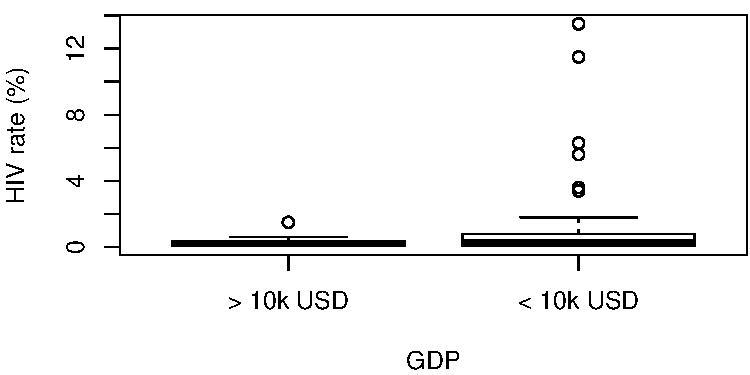
\includegraphics[width=0.75\textwidth]{Rplot-test-two-group.pdf}\end{center}

\framebreak

以\texttt{Continent}分組對\texttt{Age.ave}之描述:
\begin{RC}
> with(mydt0, {tapply(Age.ave, Continent, mean)})
\end{RC}
\begin{R}
 1Africa 2America    3Asia  4Europe 
61.11923 74.48475 72.31782 77.37283 
\end{R}
\begin{RC}
> with(mydt0, {tapply(Age.ave, Continent, sd)})
\end{RC}
\begin{R}
 1Africa 2America    3Asia  4Europe 
9.308895 4.014003 6.383229 3.820449
\end{R}

\framebreak

以\texttt{Continent}分組對\texttt{Age.ave}進行單因子變異數分析:
\begin{RC}
> f.anova <- aov(Age.ave ~ Continent, data = mydt0)
> summary(f.anova)
\end{RC}
\begin{R}
            Df Sum Sq Mean Sq F value   Pr(>F)    
Continent    3   2439   813.0   24.12 9.66e-11 ***
Residuals   68   2292    33.7                     
\end{R}

\begin{flushleft}
\scriptsize 註:此例之間間變方甚不同質,故以\nbs\verb+oneway.test(Age.ave ~ Continent, data = mydt0)+\nbs{}進行組間變方不同質之修正,或是以\nbs\verb+kruskal.test(Age.ave ~ Continent, data = mydt0)+\nbs{}進行Kruskal-Wallis rank sum test,可能較洽當。
\end{flushleft}

\framebreak

Tukey事後檢驗:
\begin{RC}
> TukeyHSD(f.anova, "Continent")
\end{RC}
\begin{R}
  Tukey multiple comparisons of means
    95% family-wise confidence level

Fit: aov(formula = Age.ave ~ Continent, data = mydt0)

$Continent
                      diff        lwr       upr     p adj
2America-1Africa 13.365519  7.2440030 19.487035 0.0000014
3Asia-1Africa    11.198593  5.5646064 16.832579 0.0000102
4Europe-1Africa  16.253603 11.1760641 21.331141 0.0000000
3Asia-2America   -2.166926 -7.9324031  3.598550 0.7556740
4Europe-2America  2.888083 -2.3349728  8.111139 0.4693185
4Europe-3Asia     5.055010  0.4129029  9.697117 0.0275116
\end{R}

\framebreak

以\nbs\verb+Continent+\nbs{}分組對\nbs\verb+Age.ave+\nbs{}繪製盒形圖:
\begin{RC}
> boxplot(Age.ave ~ Continent, data = mydt0,
+         xlab = "Continent", ylab = "Average of age",
+         xaxt = "n")
> axis(1, 1:4, 
+      label = c("Africa", "America", "Asia", "Europe"))
\end{RC}
%pdf("Rplot-test-anova.pdf", width=5, height=2.5)
%par(mar=c(4,4,0.5,0.1))
%boxplot(Age.ave ~ Continent, data = mydt0,
%        xlab = "Continent", ylab = "Average of age",
%        xaxt = "n")
%axis(1, 1:4, label = c("Africa", "America", "Asia", "Europe"))
%dev.off()
\begin{center}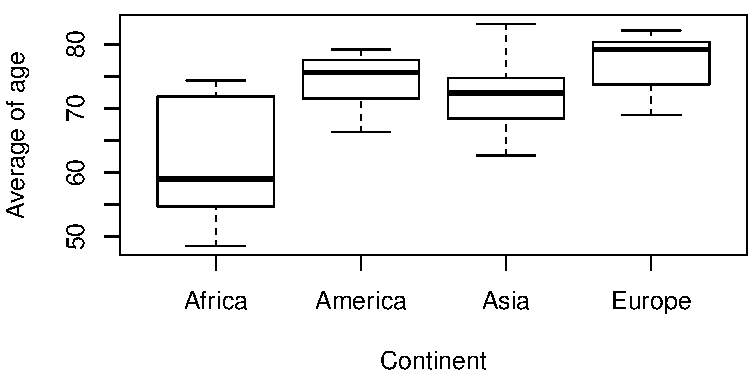
\includegraphics[width=0.75\textwidth]{Rplot-test-anova.pdf}\end{center}

\verb+HIV.rate+ vs \verb+Age.ave+ 的簡單線性迴歸:
\begin{RC}
> fit.reg <- lm(HIV.rate ~ Age.ave, data = mydt0)
> summary(fit.reg)
\end{RC}
\begin{R}
Call:
lm(formula = HIV.rate ~ Age.ave, data = mydt0)
Residuals:
    Min      1Q  Median      3Q     Max 
-2.6995 -0.8609 -0.0631  0.7118  7.8572 
Coefficients:
            Estimate Std. Error t value Pr(>|t|)    
(Intercept) 15.09700    1.73463   8.703 9.27e-13 ***
Age.ave     -0.19488    0.02369  -8.225 7.03e-12 ***
---
Residual standard error: 1.63 on 70 degrees of freedom
Multiple R-squared:  0.4915,	Adjusted R-squared:  0.4842 
F-statistic: 67.65 on 1 and 70 DF,  p-value: 7.027e-12
\end{R}

\begin{flushleft}
\scriptsize 註:考慮應變數轉型\nbs\verb!lm(sqrt(HIV.rate + 1) ~ Age.ave, ...)!\nbs{}或自變數包括二次式\nbs\verb!lm(HIV.rate ~ Age.ave + I(Age.ave ^ 2), ...)!。
\end{flushleft}

\framebreak

\verb+HIV.rate+ vs \verb+Age.ave+\nbs{}的簡單線性相關:
\begin{RC}
> cor.test( ~ HIV.rate + Age.ave, data = mydt0)
> cor.test(mydt0$HIV.rate, mydt0$Age.ave)  # 亦可
\end{RC}
\begin{R}
	Pearson's product-moment correlation

data:  mydt0$HIV.rate and mydt0$Age.ave
t = -8.2253, df = 70, p-value = 7.027e-12
alternative hypothesis: true correlation is not equal to 0
95 percent confidence interval:
 -0.8024053 -0.5604066
sample estimates:
       cor 
-0.7010578 
\end{R}

\begin{flushleft}
\scriptsize 註:考慮無母數相關\nbs\verb!cor.test(..., method = "kendall")!\nbs{}或\nbs\verb!cor.test(..., method = "spearman")!。
\end{flushleft}

\framebreak

\verb+HIV.rate+ vs \verb+Age.ave+\nbs{}的散佈圖:
\begin{RC}
> plot(HIV.rate ~ Age.ave, data = mydt0,
+      xlab = "Average of age", ylab = "HIV rate (%)")
> abline(a = coef(fit.reg)[1], b = coef(fit.reg)[2],
+        lty = 2, col = 6)
\end{RC}
\begin{center}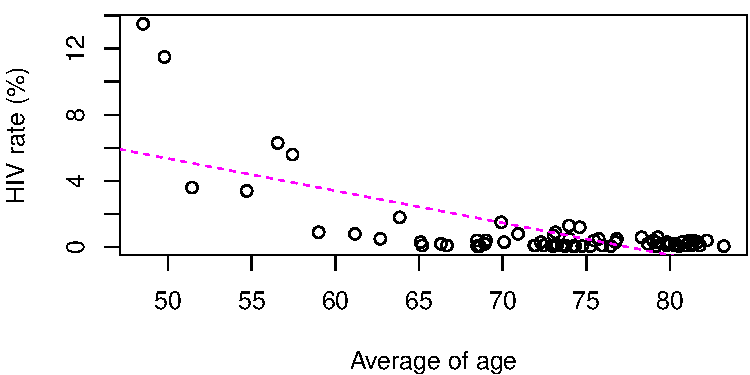
\includegraphics[width=0.75\textwidth]{Rplot-test-lm.pdf}\end{center}
%pdf("Rplot-test-lm.pdf", width=5, height=2.5)
%par(mar=c(4,4,0.5,0.1))
%plot(HIV.rate ~ Age.ave, data = mydt0,
%        xlab = "Average of age", ylab = "HIV rate (%)")
%abline(a = coef(fit.reg)[1], b = coef(fit.reg)[2], lty = 2, col = 6)
%dev.off()

\end{frame}


\end{document}